
\part{Ejercicio 1}
%aca va el ejercicio

Se implementaron dos compuertas NOT con tecnolog�a BJT: una variante con un transistor NPN (BC337) y otra con un transistor PNP (BC557). Sus dise�os se pueden observar en la siguiente figura.

%insertar referencias a figuras de dise�o
\begin{figure}[H]% este es para caption arriba o abajo
  \centering
    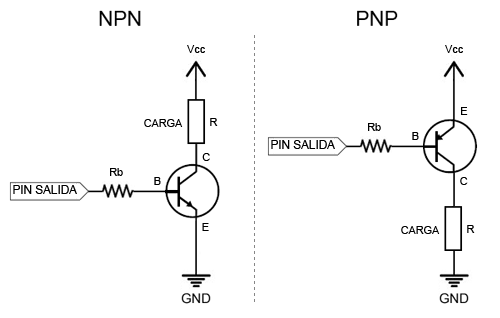
\includegraphics[width=0.5\textwidth]{circuitos}
    \caption{Circuitos inversores para transistores NPN y PNP.} %caption abajo
\end{figure}

Midiendo con un osciloscopio la entrada y la salida del circuito y haciendo uso del modo XY, se obtuvo la curva caracter\'istica de tensi\'on de cada compuerta.

A partir de estas curvas, se obtuvieron los niveles de voltaje de input y output para los niveles altos y bajos de ambas compuertas, as\'i como los m\'argenes de ruido. Estos figuran en la siguiente tabla.
\begin{center}
\begin{table}[H]
\begin{tabular}{|l|l|l|}
\hline
                          & NPN   & PNP    \\
High Level Input Voltage  & 1.18V & 4.28V  \\
Low Level Input Voltage   & 518mV & 3.08V  \\
High Level Output Voltage & 4.88V & 4.53V  \\
Low Level Output Voltage  & 462mV & 12.5mV \\
High Noise Margin         & 3.7V  & 0.25V  \\
Low Noise Margin          & 56mV  & 3.067V
\end{tabular}
\end{table}
\end{center}
Posteriormente, midiendo las curvas de entrada y salida en simult\'aneo, se obtuvieron los tiempos de transici\'on y las demoras de propagaci\'on para ambas compuertas. Luego, se cargaron las compuertas con un capacitor de 10nF, y obteniendo la derivada de la tensi�n de salida, utilizando la ley de Ohm para capacitores pudo determinarse la corriente m\'axima a trav\'es de la compuerta. Estos datos figuran en la siguiente tabla.
\begin{center}
\begin{table}[H]
\begin{tabular}{|l|l|l|}
\hline
                                       & \textbf{NPN} & \textbf{PNP} \\ \hline
\textbf{Propagation Delay High to Low} & 270 ns       & 860 ns       \\ \hline
\textbf{Propagation Delay Low to High} & 3.22 �s      & 101 ns       \\ \hline
\textbf{Transition Time High to Low}   & 230 ns       & 538 ns       \\ \hline
\textbf{Transition Time Low to High}   & 840 ns       & 159 ns       \\ \hline
\textbf{Max Output Current}            & 14.68mA      & 9.25mA       \\ \hline
\end{tabular}
\end{table}
\end{center}

\subsubsection{Mediciones en osciloscopio}
\begin{multicols}{2}
\begin{center}
\begin{figure}[H]% este es para caption arriba o abajo
  \centering
    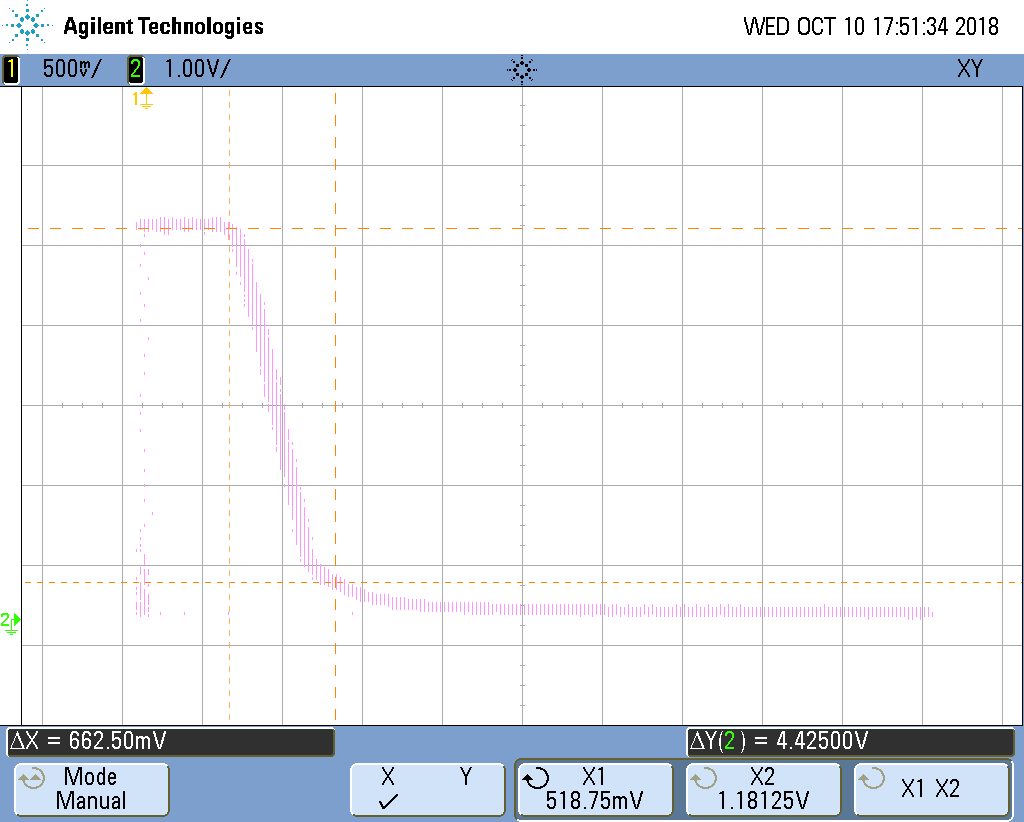
\includegraphics[width=0.4\textwidth]{ejercicio1/scope_x_Punto1_NPN}
    \caption{Curva caracter\'istica NPN: datos de input.} %caption abajo
\end{figure}

\begin{figure}[H]% este es para caption arriba o abajo
  \centering
    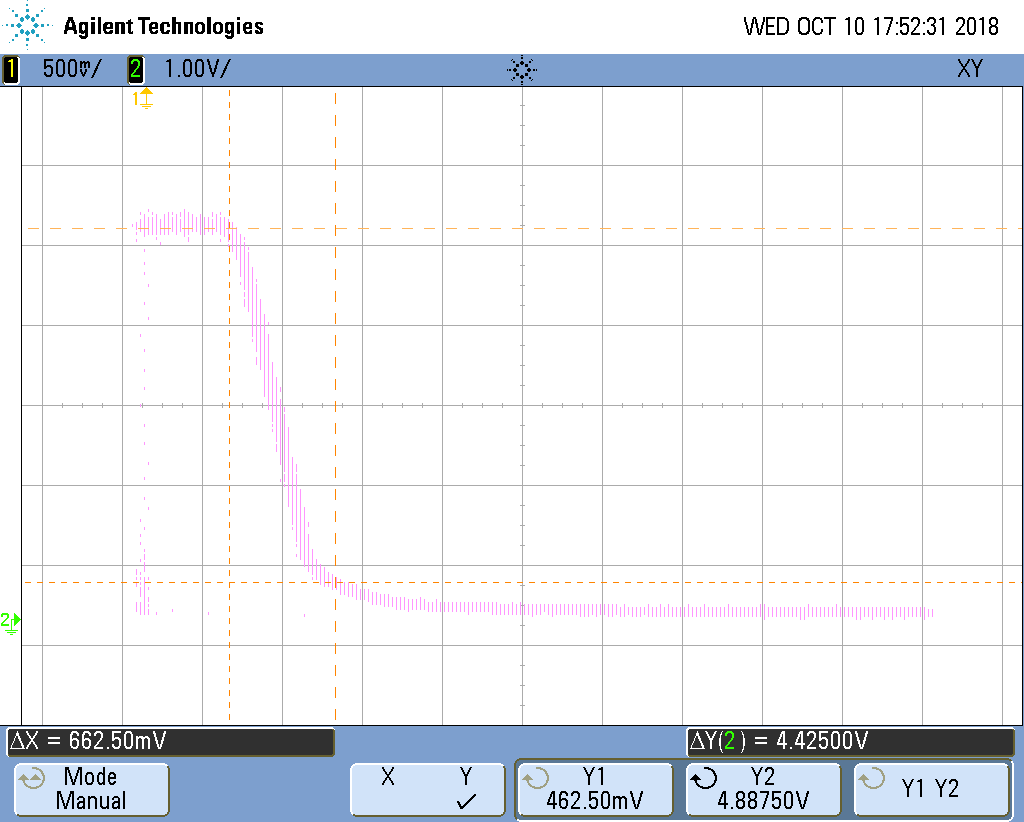
\includegraphics[width=0.4\textwidth]{ejercicio1/scope_y_Punto1_NPN}
    \caption{Curva caracter\'istica NPN: datos de output.} %caption abajo
\end{figure}

\begin{figure}[H]% este es para caption arriba o abajo
  \centering
    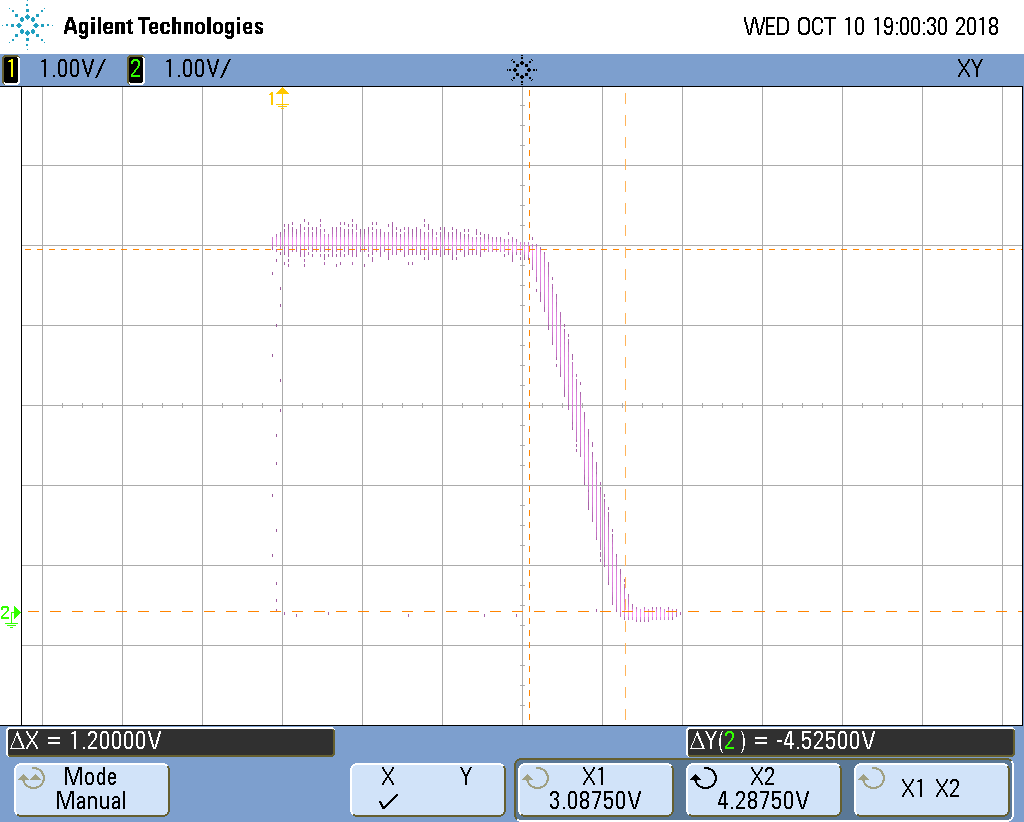
\includegraphics[width=0.4\textwidth]{ejercicio1/scope_x_Punto1_PNP}
    \caption{Curva caracter\'istica PNP: datos de input.} %caption abajo
\end{figure}

\begin{figure}[H]% este es para caption arriba o abajo
  \centering
    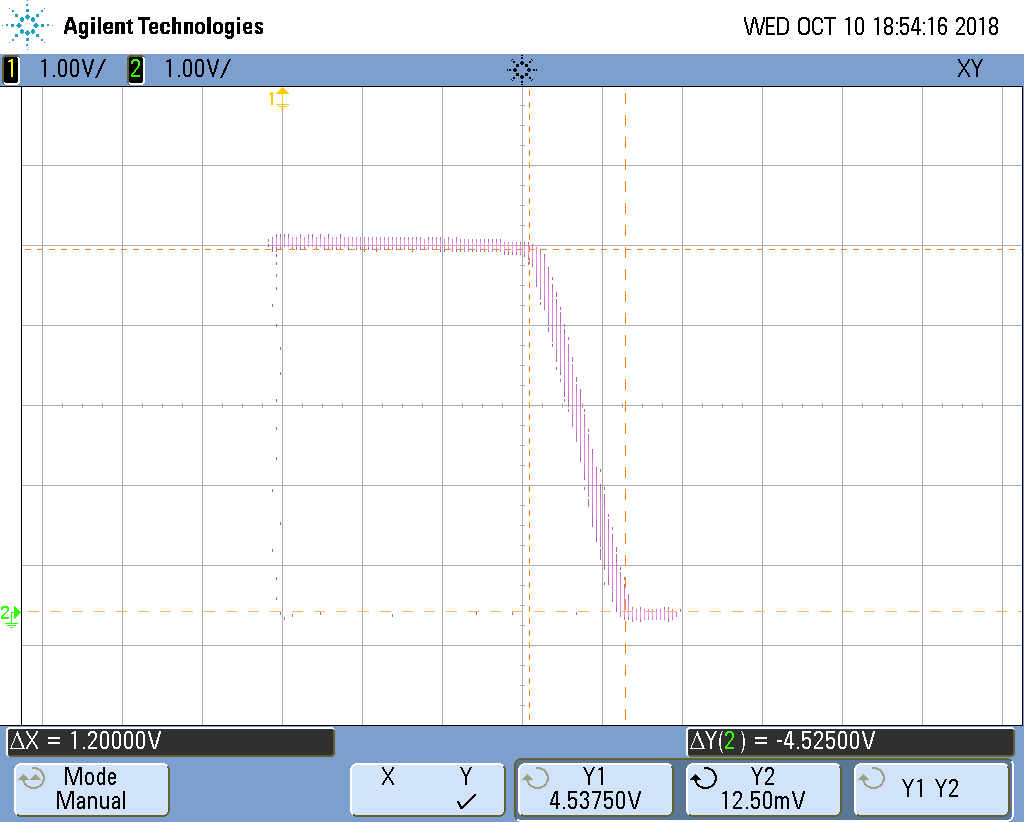
\includegraphics[width=0.4\textwidth]{ejercicio1/scope_y_Punto1_PNP}
    \caption{Curva caracter\'istica PNP: datos de output.} %caption abajo
\end{figure}

\begin{figure}[H]% este es para caption arriba o abajo
  \centering
    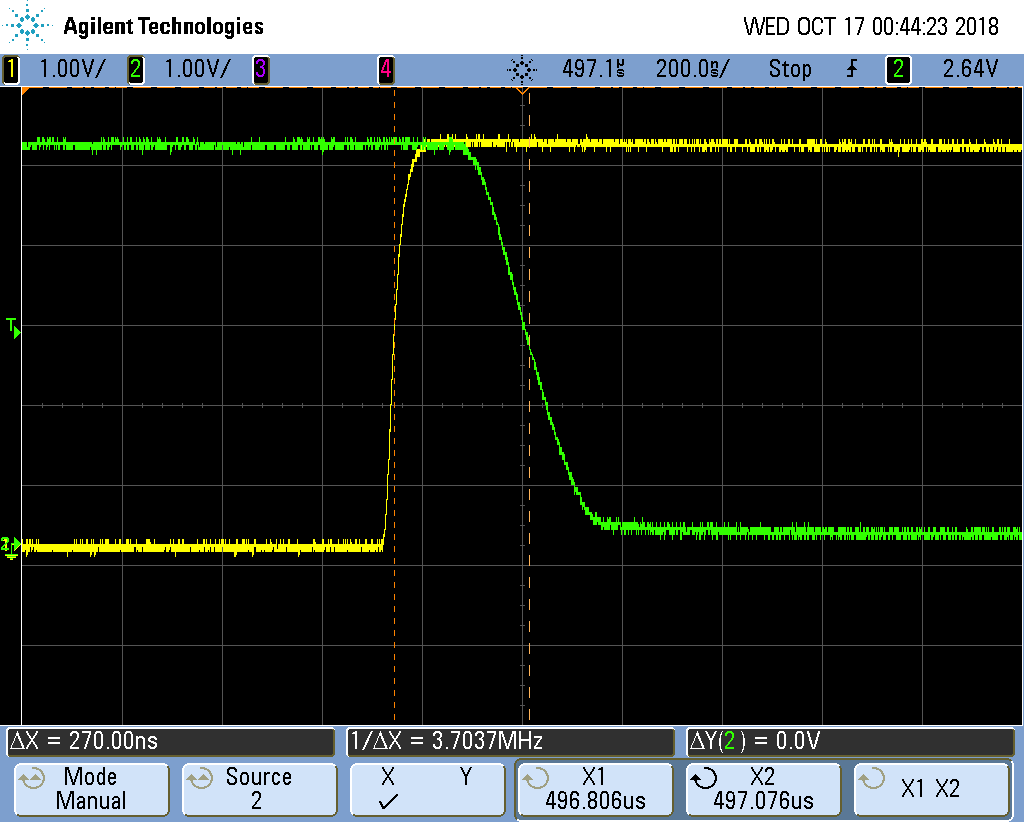
\includegraphics[width=0.4\textwidth]{ejercicio1/pHL-NPN}
    \caption{Medici\'on Propagation Delay NPN: High to Low} %caption abajo
\end{figure}

\begin{figure}[H]% este es para caption arriba o abajo
  \centering
    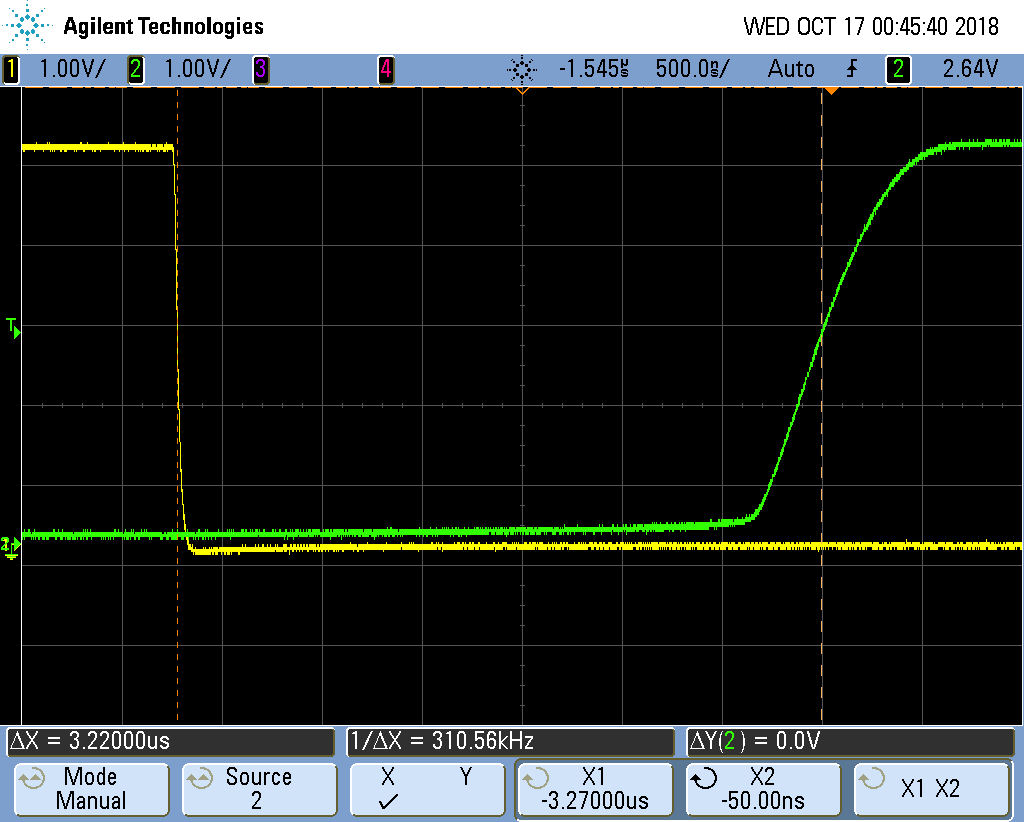
\includegraphics[width=0.4\textwidth]{ejercicio1/pLH-NPN}
    \caption{Medici\'on Propagation Delay NPN: Low to High} %caption abajo
\end{figure}

\begin{figure}[H]% este es para caption arriba o abajo
  \centering
    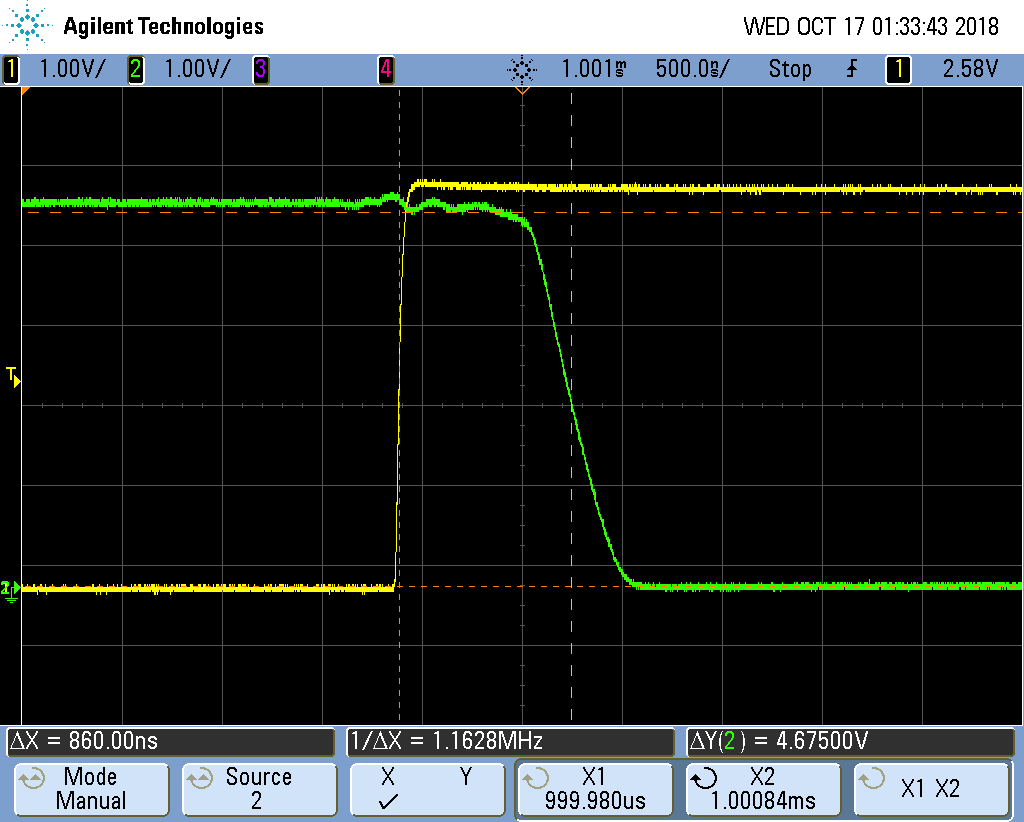
\includegraphics[width=0.4\textwidth]{ejercicio1/pHL-PNP}
    \caption{Medici\'on Propagation Delay PNP: High to Low} %caption abajo
\end{figure}

\begin{center}
\begin{figure}[H]% este es para caption arriba o abajo
  \centering
    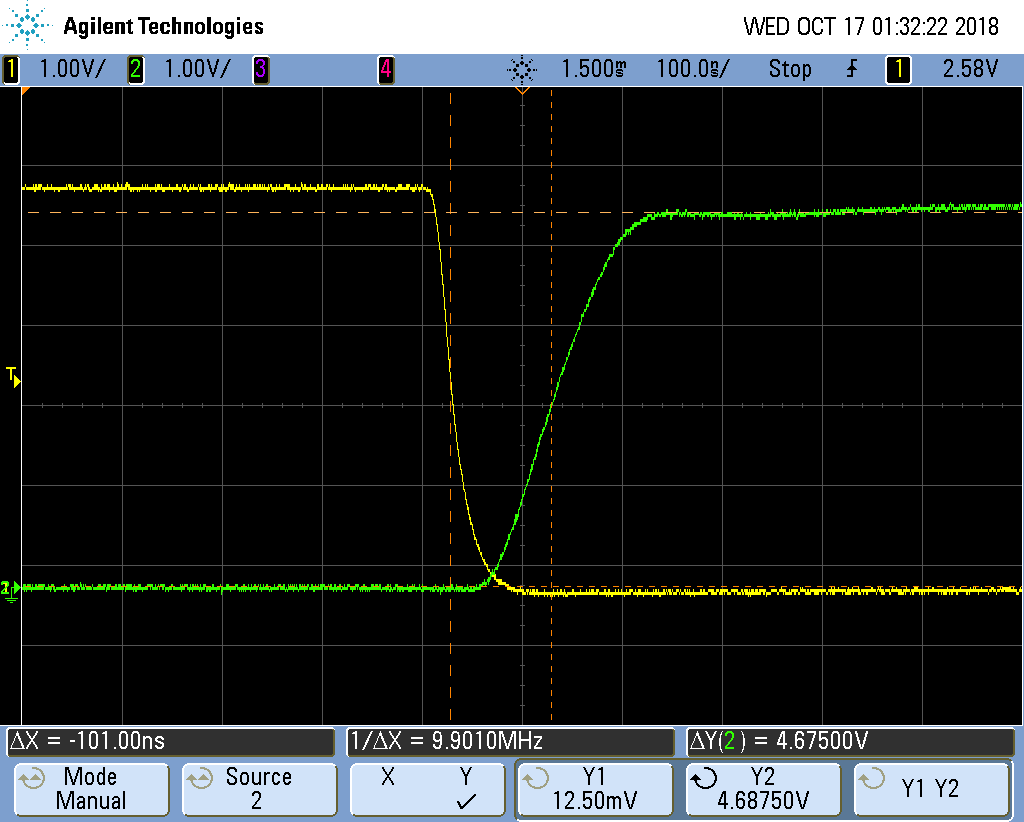
\includegraphics[width=0.4\textwidth]{ejercicio1/pLH-PNP}
    \caption{Medici\'on Propagation Delay PNP: Low to High} %caption abajo
\end{figure}

\begin{figure}[H]% este es para caption arriba o abajo
  \centering
    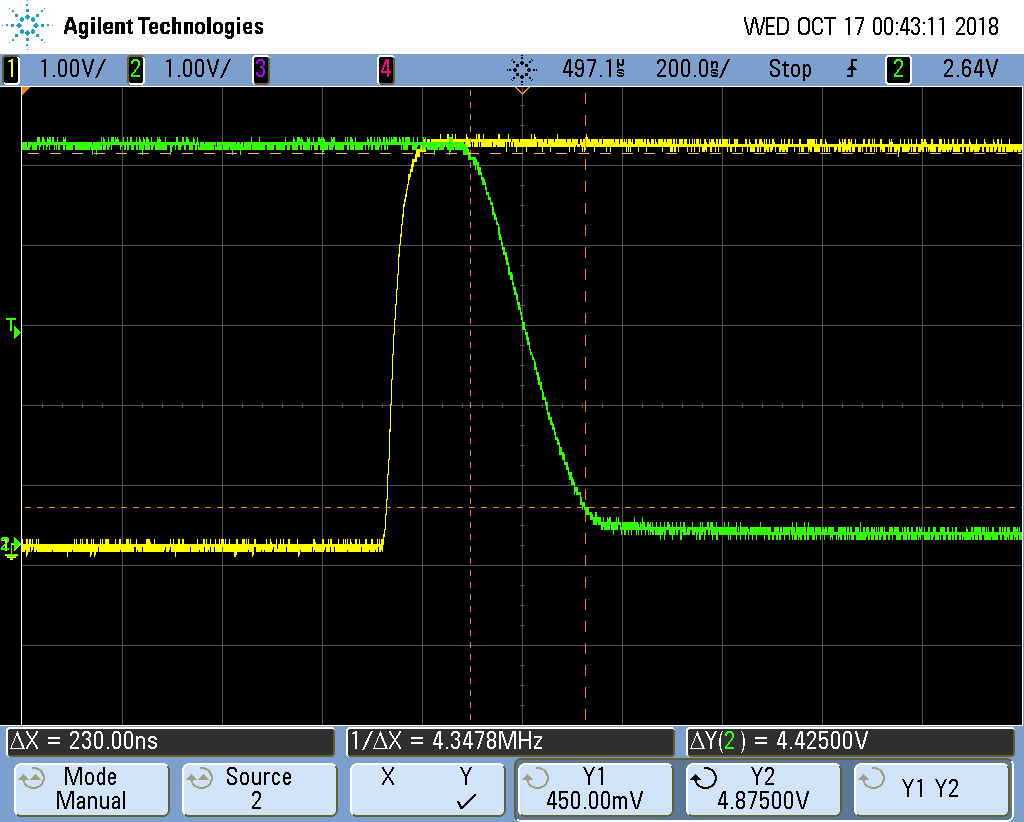
\includegraphics[width=0.4\textwidth]{ejercicio1/tHL-NPN}
    \caption{Medici\'on Transition Time NPN: High to Low} %caption abajo
\end{figure}

\begin{figure}[H]% este es para caption arriba o abajo
  \centering
    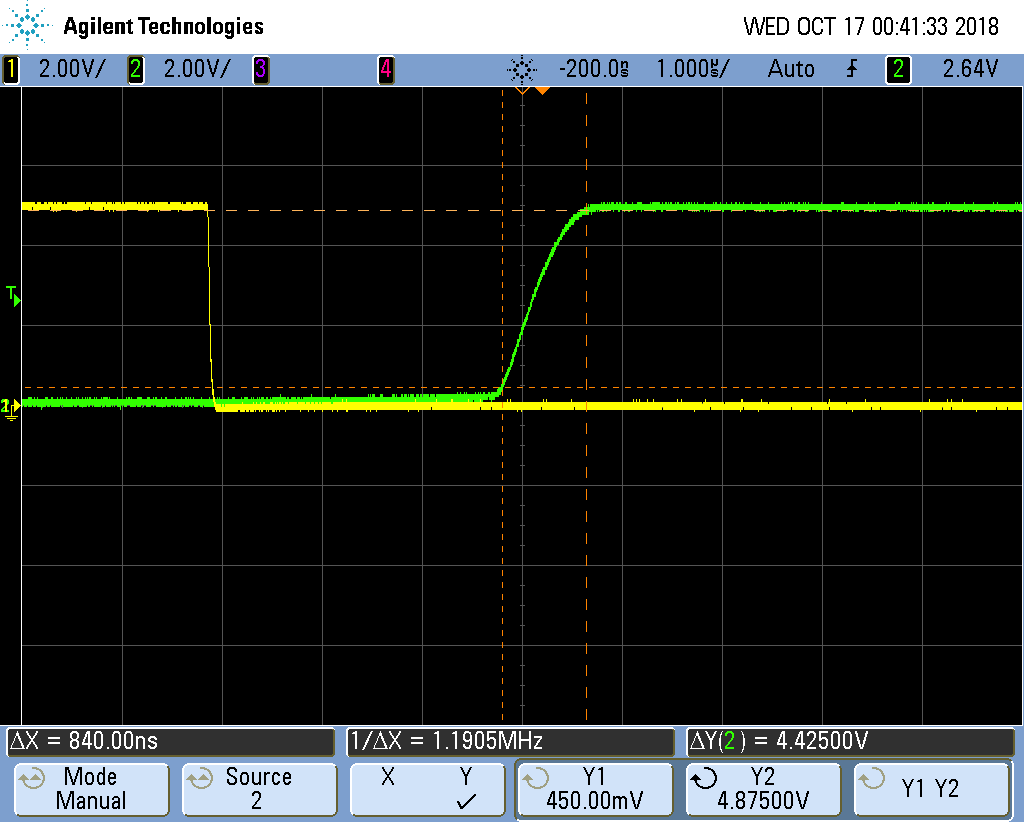
\includegraphics[width=0.4\textwidth]{ejercicio1/tLH-NPN}
    \caption{Medici\'on Transition Time NPN: Low to High} %caption abajo
\end{figure}

\begin{figure}[H]% este es para caption arriba o abajo
  \centering
    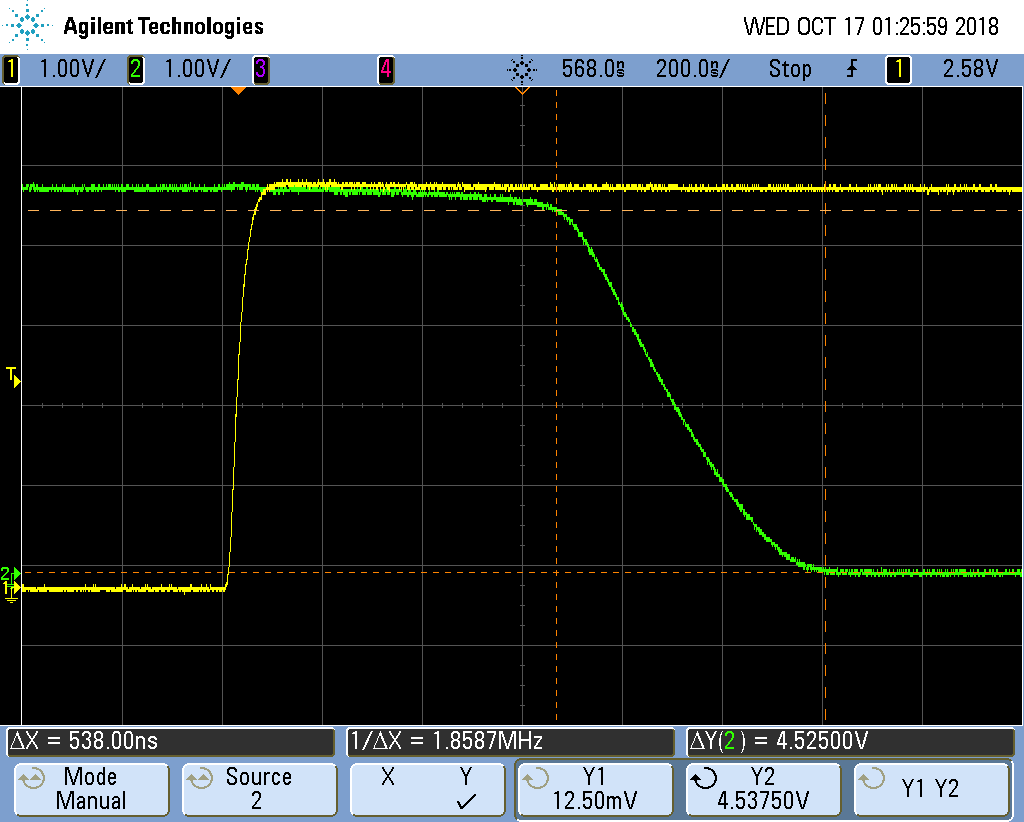
\includegraphics[width=0.4\textwidth]{ejercicio1/tHL-PNP}
    \caption{Medici\'on Transition Time PNP: High to Low} %caption abajo
\end{figure}

\begin{figure}[H]% este es para caption arriba o abajo
  \centering
    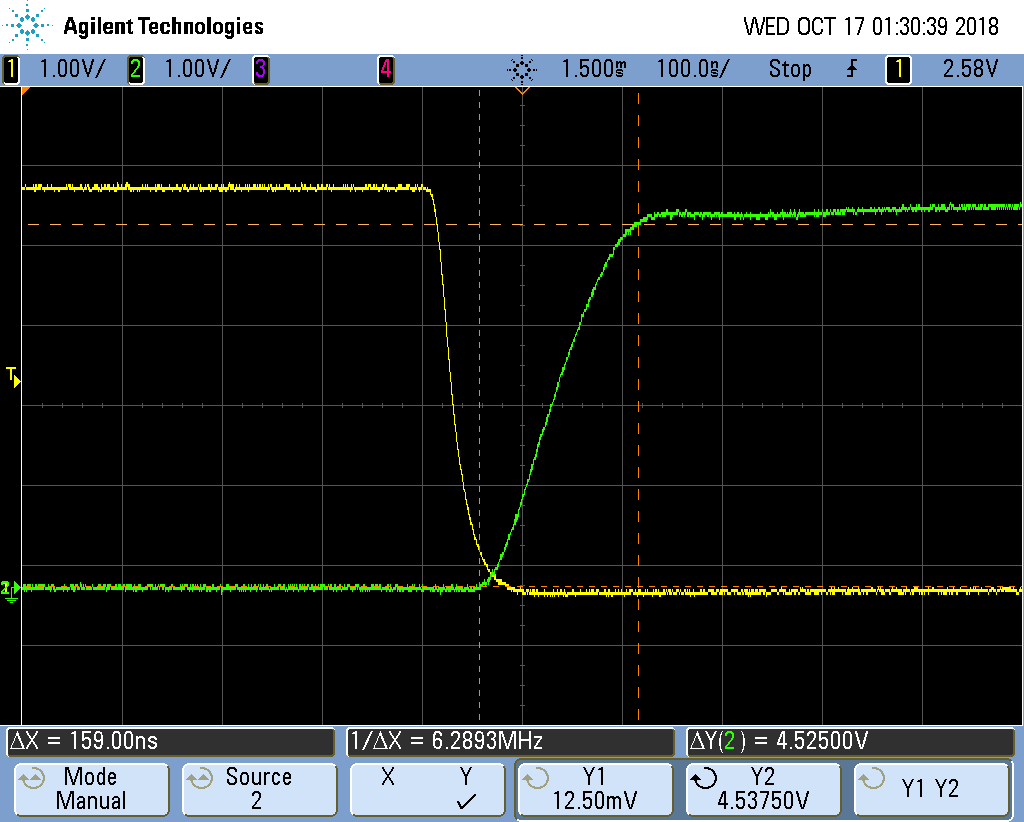
\includegraphics[width=0.4\textwidth]{ejercicio1/tLH-PNP}
    \caption{Medici\'on Transition Time PNP: Low to High} %caption abajo
\end{figure}

\begin{figure}[H]% este es para caption arriba o abajo
  \centering
    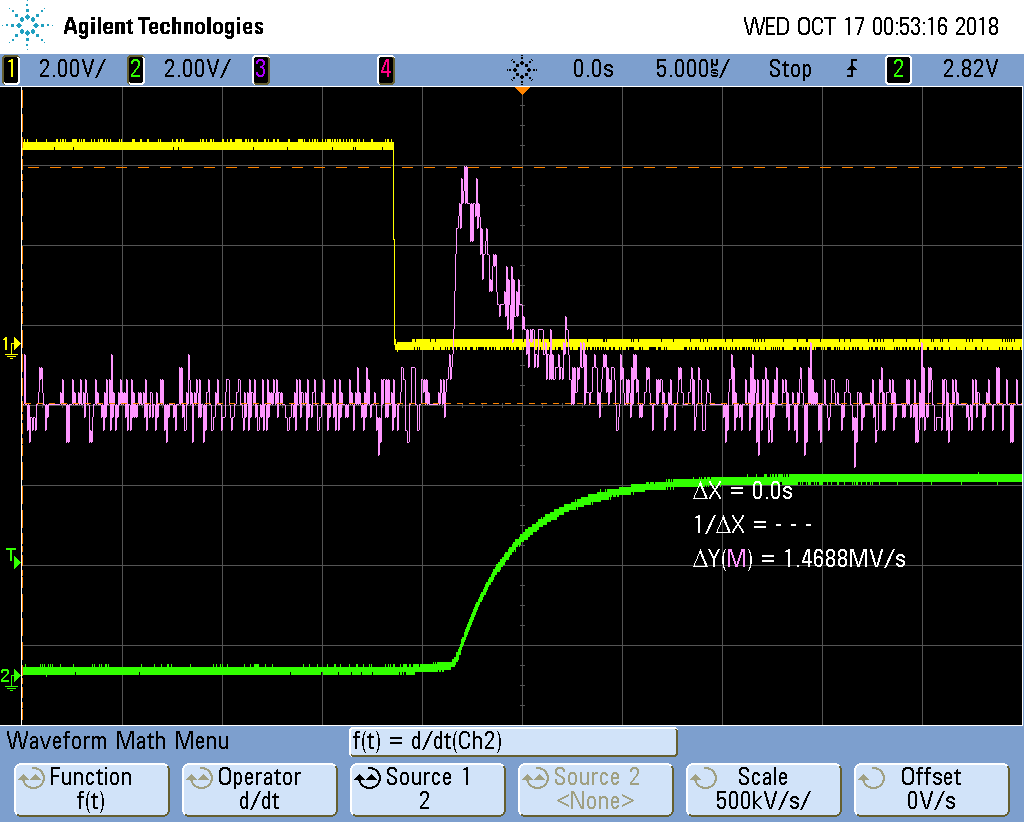
\includegraphics[width=0.4\textwidth]{ejercicio1/maxI-NPN}
    \caption{Medici\'on m�xima derivada de tensi�n en la salida NPN} %caption abajo
\end{figure}

\begin{figure}[H]% este es para caption arriba o abajo
  \centering
    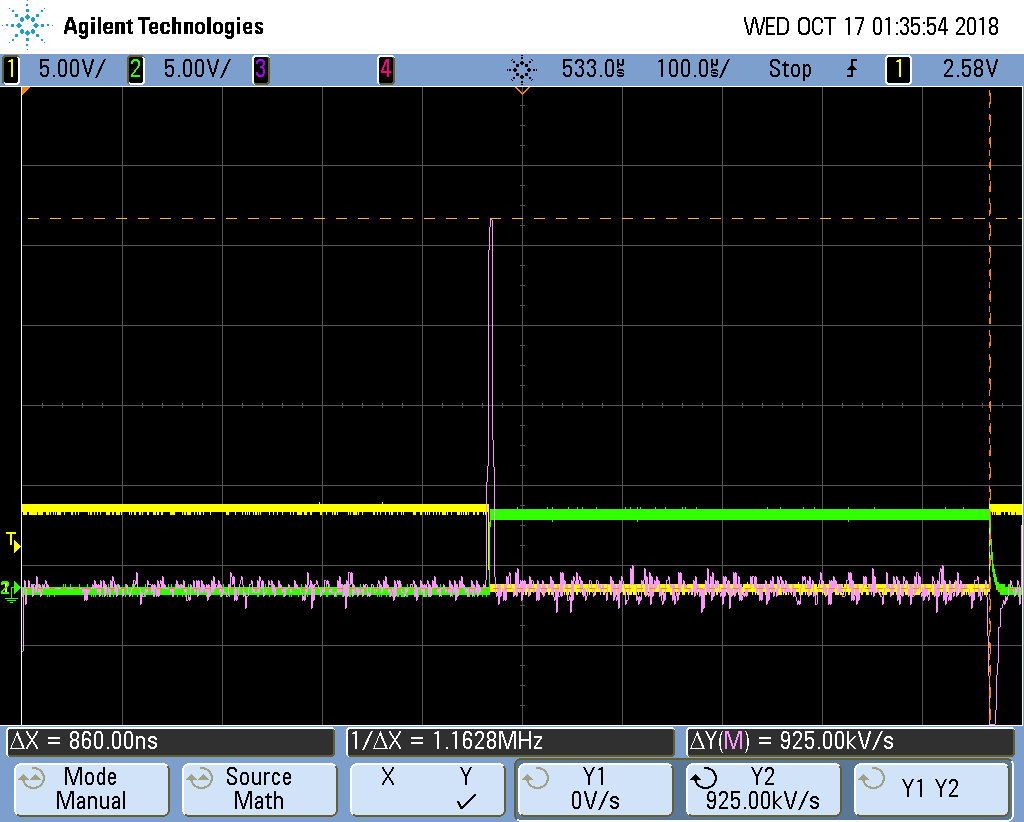
\includegraphics[width=0.4\textwidth]{ejercicio1/maxI-PNP}
    \caption{Medici\'on m�xima derivada de tensi�n en la salida PNP} %caption abajo
\end{figure}
\end{center}
\end{multicols}
\iffalse
Seccion de cosas utiles para agregar

texto----------------------------
\textit[texto en negrita]




listas --------------------------------------------------
\begin{list_type}  
\item The first item 
\item The second item 
\item The third etc \ldots 
\end{list_type}

list_type es:
itemize for a bullet list
enumerate for an enumerated list and
description for a descriptive list.

ejemplo listas anidadas-----------------------------------------------

\begin{enumerate}
\item The first item
\begin{enumerate}
\item Nested item 1
\item Nested item 2
\end{enumerate}
\item The second item
\item The third etc \ldots
\end{enumerate}

tildes-------------------------------
babel ya esta incluido, si hay que poner tildes se ponen \acute{i}
ejemplo: l\acute{i}mite

tip: escriban normal y despues hagan replace

subsecciones-------------------------------

si necesitan subsecciones le clavan un buen \subsection*{nombre}

y si estan en piolas y necesitan sub sub secciones le clavan un \subsubsection*{nombre}

quien hubiera dicho

figuras----------------------------------------

\begin{figure}% este es para caption arriba o abajo
  \caption{A picture of a gull.} %caption arriba
  \centering
    \includegraphics[width=0.5\textwidth]{ejercicio1/gull}
    \caption{A picture of a gull.} %caption abajo
\end{figure}

\begin{SCfigure} %este es para caption al costado
  \centering
  \caption{ ... caption text ... } 
  \includegraphics[width=0.3\textwidth]%
    {ejercicio1/Giraffe_picture}% picture filename
\end{SCfigure}

para hacer que la figure se quede quietecita:

\begin{figure}[letrita_placement]

donde letrita_placement es:
h	Place the float here, i.e., approximately at the same point it occurs in the source text (however, not exactly at the spot)
t	Position at the top of the page.
b	Position at the bottom of the page.
p	Put on a special page for floats only.
!	Override internal parameters LaTeX uses for determining "good" float positions.
H	Places the float at precisely the location in the LaTeX code. Requires the float package,[1] i.e., \usepackage{float}. This is somewhat equivalent to !ht.

\fi